
\documentclass[oneside,letterpaper,12pt]{book}
\usepackage{Rd}
%\usepackage{Sweave}
%\usepackage{/usr/lib64/R/share/texmf/Sweave}
%\usepackage{/usr/share/R/texmf/Sweave}
\usepackage{bibentry}
\usepackage{upquote}
\usepackage{graphicx}
\usepackage{natbib}
\usepackage[reqno]{amsmath}
\usepackage{amssymb}
\usepackage{amsfonts}
\usepackage{amsmath}
\usepackage{verbatim}
\usepackage{epsf}
\usepackage{url}
\usepackage{html}
\usepackage{dcolumn}
\usepackage{multirow}
\usepackage{fullpage}
\usepackage{lscape}
\usepackage[all]{xy}

\usepackage{csquotes}
% \usepackage[pdftex, bookmarksopen=true,bookmarksnumbered=true,
%   linkcolor=webred]{hyperref}
\bibpunct{(}{)}{;}{a}{}{,}
\newcolumntype{.}{D{.}{.}{-1}}
\newcolumntype{d}[1]{D{.}{.}{#1}}
\htmladdtonavigation{
  \htmladdnormallink{%
    \htmladdimg{http://gking.harvard.edu/pics/home.gif}}
  {http://gking.harvard.edu/}}
\newcommand{\MatchIt}{{\sc MatchIt}}
\newcommand{\hlink}{\htmladdnormallink}
\newcommand{\Sref}[1]{Section~\ref{#1}}
\newcommand{\fullrvers}{2.5.1}
\newcommand{\rvers}{2.5}
\newcommand{\rwvers}{R-2.5.1}
%\renewcommand{\bibentry}{\citealt}

\bodytext{ BACKGROUND="http://gking.harvard.edu/pics/temple.jpg"}
\setcounter{tocdepth}{2}

%\VignetteIndexEntry{Least Squares Regression for Continuous Dependent Variables}
%\VignetteDepends{Zelig, stats}
%\VignetteKeyWords{model,least squares,continuous, regression}
%\VignettePackage{Zelig}
\usepackage{Sweave}
\begin{document}
\nobibliography*


\section{{\tt ls}: Least Squares Regression for Continuous
Dependent Variables}
\label{ls}

Use least squares regression analysis to estimate the best linear
predictor for the specified dependent variables.

\subsubsection{Syntax}

\begin{verbatim}
> z.out <- zelig(Y ~ X1 + X2, model = "ls", data = mydata)
> x.out <- setx(z.out)
> s.out <- sim(z.out, x = x.out)
\end{verbatim}

\subsubsection{Additional Inputs}  

In addition to the standard inputs, {\tt zelig()} takes the following
additional options for least squares regression:  
\begin{itemize}
\item {\tt robust}: defaults to {\tt FALSE}.  If {\tt TRUE} is
selected, {\tt zelig()} computes robust standard errors based on
sandwich estimators (see \cite{Zeileis04}, \cite{Huber81}, and
\cite{White80}).  The default type of robust standard error is
heteroskedastic consistent (HC), \emph{not} heteroskedastic and
autocorrelation consistent (HAC).  

In addition, {\tt robust} may be a list with the following options:  
\begin{itemize}
\item {\tt method}:  choose from 
\begin{itemize}
\item {\tt "vcovHC"}: (the default if {\tt robust = TRUE}), HC standard errors.
\item {\tt "vcovHAC"}: HAC standard errors without weights.  
\item {\tt "kernHAC"}: HAC standard errors using the weights given in
\cite{Andrews91}.   
\item {\tt "weave"}: HAC standard errors using the weights given in
\cite{LumHea99}.
\end{itemize} 
\item {\tt order.by}: only applies to the HAC methods above.  Defaults to
{\tt NULL} (the observations are chronologically ordered as in the
original data).  Optionally, you may specify a time index (either as
{\tt order.by = z}, where {\tt z} exists outside the data frame; or
as {\tt order.by = \~{}z}, where {\tt z} is a variable in the data
frame).  The observations are chronologically ordered by the size of
{\tt z}.
\item {\tt \dots}:  additional options passed to the functions
specified in {\tt method}.  See the {\tt sandwich} library and
\cite{Zeileis04} for more options.   
\end{itemize}
\end{itemize}

\subsubsection{Examples}
\begin{enumerate}
\item Basic Example with First Differences

Attach sample data:
\begin{Schunk}
\begin{Sinput}
> data(macro)
\end{Sinput}
\end{Schunk}
Estimate model:
\begin{Schunk}
\begin{Sinput}
> z.out1 <- zelig(unem ~ gdp + capmob + trade, model = "ls", data = macro)
\end{Sinput}
\end{Schunk}
Summarize regression coefficients:
\begin{Schunk}
\begin{Sinput}
> summary(z.out1)
\end{Sinput}
\end{Schunk}
Set explanatory variables to their default (mean/mode) values, with
high (80th percentile) and low (20th percentile) values for the trade variable:
\begin{Schunk}
\begin{Sinput}
> x.high <- setx(z.out1, trade = quantile(macro$trade, 0.8))
> x.low <- setx(z.out1, trade = quantile(macro$trade, 0.2))
\end{Sinput}
\end{Schunk}
Generate first differences for the effect of high versus low trade on
GDP:
\begin{Schunk}
\begin{Sinput}
> s.out1 <- sim(z.out1, x = x.high, x1 = x.low)
\end{Sinput}
\end{Schunk}
\begin{Schunk}
\begin{Sinput}
> summary(s.out1)
\end{Sinput}
\end{Schunk}
\begin{center}
\begin{Schunk}
\begin{Sinput}
> plot(s.out1)
\end{Sinput}
\end{Schunk}
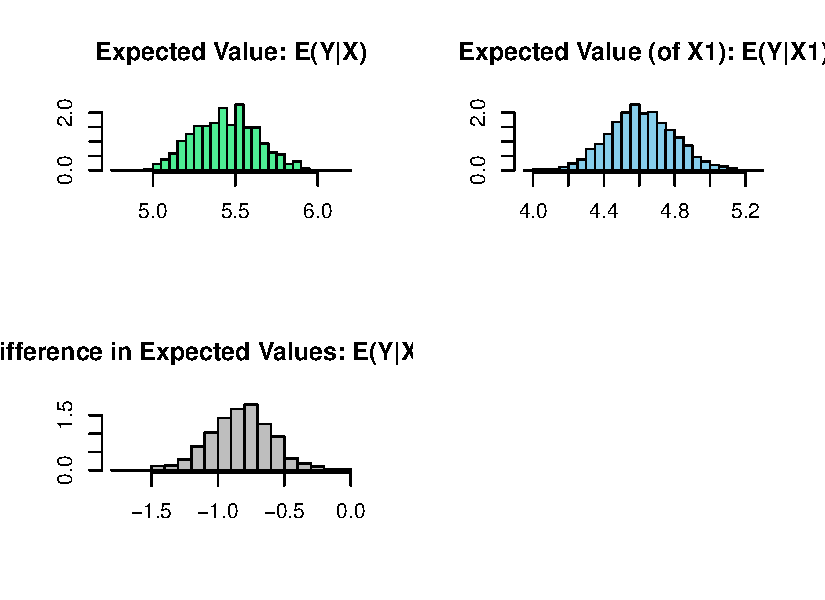
\includegraphics{vigpics/ls-ExamplesPlot}
\end{center}

\item Using Dummy Variables

Estimate a model with fixed effects for each country (see
\Sref{factors} for help with dummy variables).  Note that you do not
need to create dummy variables, as the program will automatically
parse the unique values in the selected variable into discrete levels.  
\begin{Schunk}
\begin{Sinput}
> z.out2 <- zelig(unem ~ gdp + trade + capmob + as.factor(country), 
+     model = "ls", data = macro)
\end{Sinput}
\end{Schunk}
Set values for the explanatory variables, using the default mean/mode
values, with country set to the United States and Japan, respectively:
\begin{Schunk}
\begin{Sinput}
> x.US <- setx(z.out2, country = "United States")
> x.Japan <- setx(z.out2, country = "Japan")
\end{Sinput}
\end{Schunk}
Simulate quantities of interest:
\begin{Schunk}
\begin{Sinput}
> s.out2 <- sim(z.out2, x = x.US, x1 = x.Japan)
\end{Sinput}
\end{Schunk}
\begin{center}
\begin{Schunk}
\begin{Sinput}
> plot(s.out2)
\end{Sinput}
\end{Schunk}
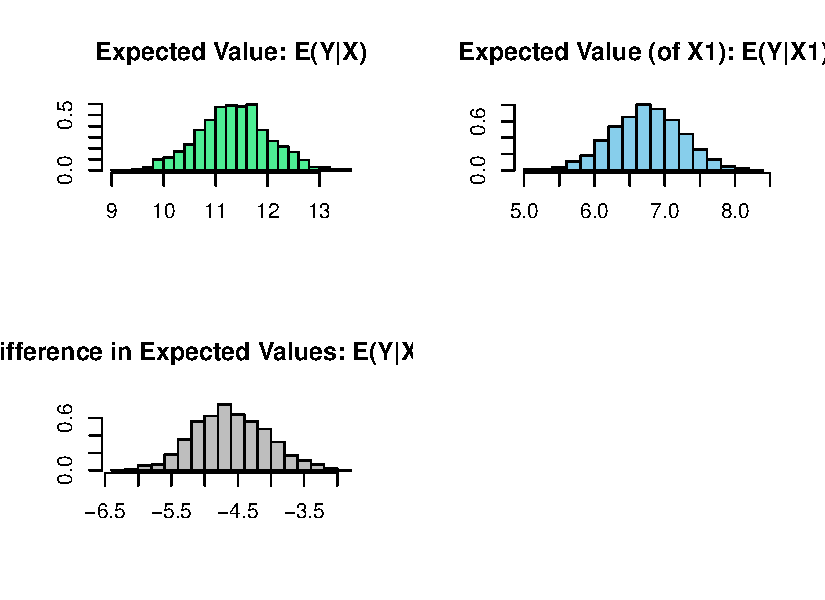
\includegraphics{vigpics/ls-DummyPlot}
\end{center}

% \item Multiple responses (least squares regression will be fitted
%   separately to each dependent variable)

% Two responses for data set macro: 
% <<Multiple.zelig>>=
%  z.out3 <- zelig(cbind(unem, gdp) ~ capmob + trade,model = "ls", data = macro)
% @
% <<Multiple.zelig.summary>>=
% summary(z.out3)
% @    
% Set values for the explanatory variables, using the default mean/mode
% values, with country set to the United States and Japan, respectively:
% <<Multiple.setx>>=
%  x.US <- setx(z.out3, country = "United States")
%  x.Japan <- setx(z.out3, country = "Japan")
% @ 
% Simulate quantities of interest:
% <<Multiple.sim>>=
%  s.out3 <- sim(z.out3, x = x.US, x1 = x.Japan)
% @
% Summary
% <<Example4.sim.summary>>=
% summary(s.out3)
% @  
% \begin{center}
% <<label=Example4Plot,fig=true,echo=true,  width=7.5, height=6>>= 
%  plot(s.out3)
% @ 
%\end{center}

\end{enumerate}

\subsubsection{Model}
\begin{itemize}
\item The \emph{stochastic component} is described by a density
  with mean $\mu_i$ and the common variance $\sigma^2$
  \begin{equation*}
    Y_i \; \sim \; f(y_i \mid \mu_i, \sigma^2).
  \end{equation*}
\item The \emph{systematic component} models the conditional mean as
  \begin{equation*}
     \mu_i =  x_i \beta
  \end{equation*} 
  where $x_i$ is the vector of covariates, and $\beta$ is the vector
  of coefficients.
  
  The least squares estimator is the best linear predictor of a
  dependent variable given $x_i$, and minimizes the sum of squared
  residuals, $\sum_{i=1}^n (Y_i-x_i \beta)^2$.  
\end{itemize}

\subsubsection{Quantities of Interest} 
\begin{itemize}
\item The expected value ({\tt qi\$ev}) is the mean of simulations
  from the stochastic component,  
\begin{equation*}
E(Y) = x_i \beta,\end{equation*}
given a draw of $\beta$ from its sampling distribution.  

\item In conditional prediction models, the average expected treatment
  effect ({\tt att.ev}) for the treatment group is 
    \begin{equation*} \frac{1}{\sum_{i=1}^n t_i}\sum_{i:t_i=1}^n \left\{ Y_i(t_i=1) -
      E[Y_i(t_i=0)] \right\},
    \end{equation*} 
    where $t_i$ is a binary explanatory variable defining the treatment
    ($t_i=1$) and control ($t_i=0$) groups.  Variation in the
    simulations are due to uncertainty in simulating $E[Y_i(t_i=0)]$,
    the counterfactual expected value of $Y_i$ for observations in the
    treatment group, under the assumption that everything stays the
    same except that the treatment indicator is switched to $t_i=0$.

\end{itemize}

\subsubsection{Output Values}

The output of each Zelig command contains useful information which you
may view.  For example, if you run \texttt{z.out <- zelig(y \~\,
  x, model = "ls", data)}, then you may examine the available
information in \texttt{z.out} by using \texttt{names(z.out)},
see the {\tt coefficients} by using {\tt z.out\$coefficients}, and
a default summary of information through \texttt{summary(z.out)}.
Other elements available through the {\tt \$} operator are listed
below.

\begin{itemize}
  \item From the {\tt zelig()} output object {\tt z.out}, you may
  extract:
   \begin{itemize}
   \item {\tt coefficients}: parameter estimates for the explanatory
     variables.
   \item {\tt residuals}: the working residuals in the final iteration
     of the IWLS fit.
   \item {\tt fitted.values}: fitted values.
   \item {\tt df.residual}: the residual degrees of freedom.
   \item {\tt zelig.data}: the input data frame if {\tt save.data = TRUE}.  
   \end{itemize}
  
\item From {\tt summary(z.out)}, you may extract:
   \begin{itemize}
   \item {\tt coefficients}: the parameter estimates with their
     associated standard errors, $p$-values, and $t$-statistics.
     \begin{equation*}
       \hat{\beta} \; = \; \left(\sum_{i=1}^n x_i' x_i\right)^{-1} \sum x_i y_i
     \end{equation*}
   \item {\tt sigma}: the square root of the estimate variance of the
     random error $e$:
     \begin{equation*}
       \hat{\sigma} \; = \; \frac{\sum (Y_i-x_i\hat{\beta})^2}{n-k}
     \end{equation*}
   \item {\tt r.squared}: the fraction of the variance explained by
     the model. 
     \begin{equation*}
       R^2 \; = \; 1 - \frac{\sum (Y_i-x_i\hat{\beta})^2}{\sum (y_i -
         \bar{y})^2} 
     \end{equation*}
   \item {\tt adj.r.squared}: the above $R^2$ statistic, penalizing
     for an increased number of explanatory variables.  
   \item{\tt cov.unscaled}: a $k \times k$ matrix of unscaled
     covariances.  
   \end{itemize}
   
\item From the {\tt sim()} output object {\tt s.out}, you may extract
  quantities of interest arranged as matrices indexed by simulation
  $\times$ {\tt x}-observation (for more than one {\tt x}-observation).
  Available quantities are:

   \begin{itemize}
   \item {\tt qi\$ev}: the simulated expected values for the specified
     values of {\tt x}.
   \item {\tt qi\$fd}:  the simulated first differences (or
     differences in expected values) for the specified values of {\tt
       x} and {\tt x1}. 
   \item {\tt qi\$att.ev}: the simulated average expected treatment
     effect for the treated from conditional prediction models.  
   \end{itemize}
\end{itemize}

\subsection* {How to Cite} 

\CiteZelig

\subsection* {See also}
The least squares regression is part of the stats package by William N.
Venables and Brian D. Ripley \citep{VenRip02}.In addition, advanced users may wish to refer to \texttt{help(lm)} and \texttt{help(lm.fit)}.Robust standard errors are implemented via the sandwich package by Achim Zeileis \citep{Zeileis04}.Sample data are from \cite{KinTomWit00}.

\bibliographystyle{asa}
\bibliography{gk,gkpubs}
 \end{document}

%%% Local Variables: 
%%% mode: latex
%%% TeX-master: t
%%% TeX-master: t
%%% End: 
